\documentclass[twocolumn,10pt]{article}

\usepackage[a4paper,hmargin=1.5cm,vmargin=2.5cm,]{geometry}
\setlength{\columnsep}{0.7cm}
\usepackage{palatino}
\usepackage{graphicx}
\usepackage[utf8]{inputenc}
\usepackage{hyperref}
\usepackage{minted}
\usemintedstyle{colorful}
\usepackage[font=small,labelfont=bf]{caption}
\urlstyle{same} % no tt font for URLs
\newcommand{\blockade}{\rule{3em}{0.7em}}  %% Marker for things to change before submission

\usepackage{natbib}
\bibliographystyle{genome_research}
\setcitestyle{aysep={}} 

\usepackage{xcolor}
\hypersetup{
    colorlinks,
    linkcolor={blue!50!black},
    citecolor={blue!50!black},
    urlcolor={blue!50!black}
}

\begin{document}

\setcounter{secnumdepth}{0}


\twocolumn[{%
\centering
\textbf{\Large R/LinkedCharts: A novel approach for simple but powerful interactive data analysis}
\vspace{1.5ex}

Svetlana Ovchinnikova and Simon Anders\\
{\footnotesize Center for Molecular Biology of the University of Heidelberg, Germany}
\vspace{1.5ex}

24 January 2020
\vspace{6ex}
}]

\section{Abstract}
In exploratory data analysis, one usually jumps back and forth between visualizations that provide overview of the whole data and others that dive into details. In data quality assessment, for example, it might be very helpful to have one chart showing a summary statistic for all samples, and clicking on one of the data points would display details on this sample in a second plot. Setting up such interactively linked charts is usually cumbersome and time-consuming to use them in ad hoc analysis. We present R/LinkedCharts, a framework  that renders this tasks radically simple: Producing linked charts is as quickly done as is producing conventional static plots in R, requiring a data scientist to write only very few lines of simple R code to obtain complex and general visualization. We expect that the convenience of our new tool will enable data scientists and bioinformaticians to perform much deeper and more thorough EDA with much less effort. Furthermore, R/LinkedCharts apps, typically first written as quick-and-dirty hacks, can also be polished to provide interactive data access in publication quality, thus contributing to open science.

\section{Introduction}
Today there are no doubts that interactivity is becoming an extremely powerful tool for data exploration and presentation. Many journals now expect authors to provide access to their data and results in the form of an interactive app. This way readers get an opportunity to check important claims of the paper directly and even to find answers to their own questions. Such apps generally provide an intuitive way to dive into the data without any need of going through software and scripts used in the paper. Another common area of interactivity application is data exploration. In recent years lots of software packages have emerged that generate interactive reports, produce interactive plots or provide other means of obtaining information about the data set in an interactive manner (some references).

Main advantage of interactivity lies beyond just simplifying navigation through big massives of data. When adding small changes to a plot takes just a click or two instead of writing some pieces of code and rerunning scripts, it urges a researcher not to put aside ideas or concerns and thus go through the data more thoroughly. At the same time a possibility for readers to check conclusions and claims of a paper on the fly, without going through all the script and analysis, makes the paper more credible. Therefore, we believe that further integration of interactive tools in a researchers' routine can strongly improve quality of studies.

To this end tools that produce interactive apps should be both simple to use and highly customizeable. One doesn't want to spend couple of days on designing an app just for some \emph{ad hoc} analysis. At the same time, software that is too specific and has too many hard-coded elements will not allow for much freedom of ideas.

Keeping these two goals in mind, we've designed LinkedCharts: a library for making interactive apps available both as R version (can be installed from CRAN) and as a JavaScript library. This paper will be concentrated on R implementation of LinkedCharts. R/LinkedCharts allows to create and share interactive apps with not more effort than it takes to make conventional static plots.

\section{Results}
\subsection{Structure and linking}
\begin{figure*}
	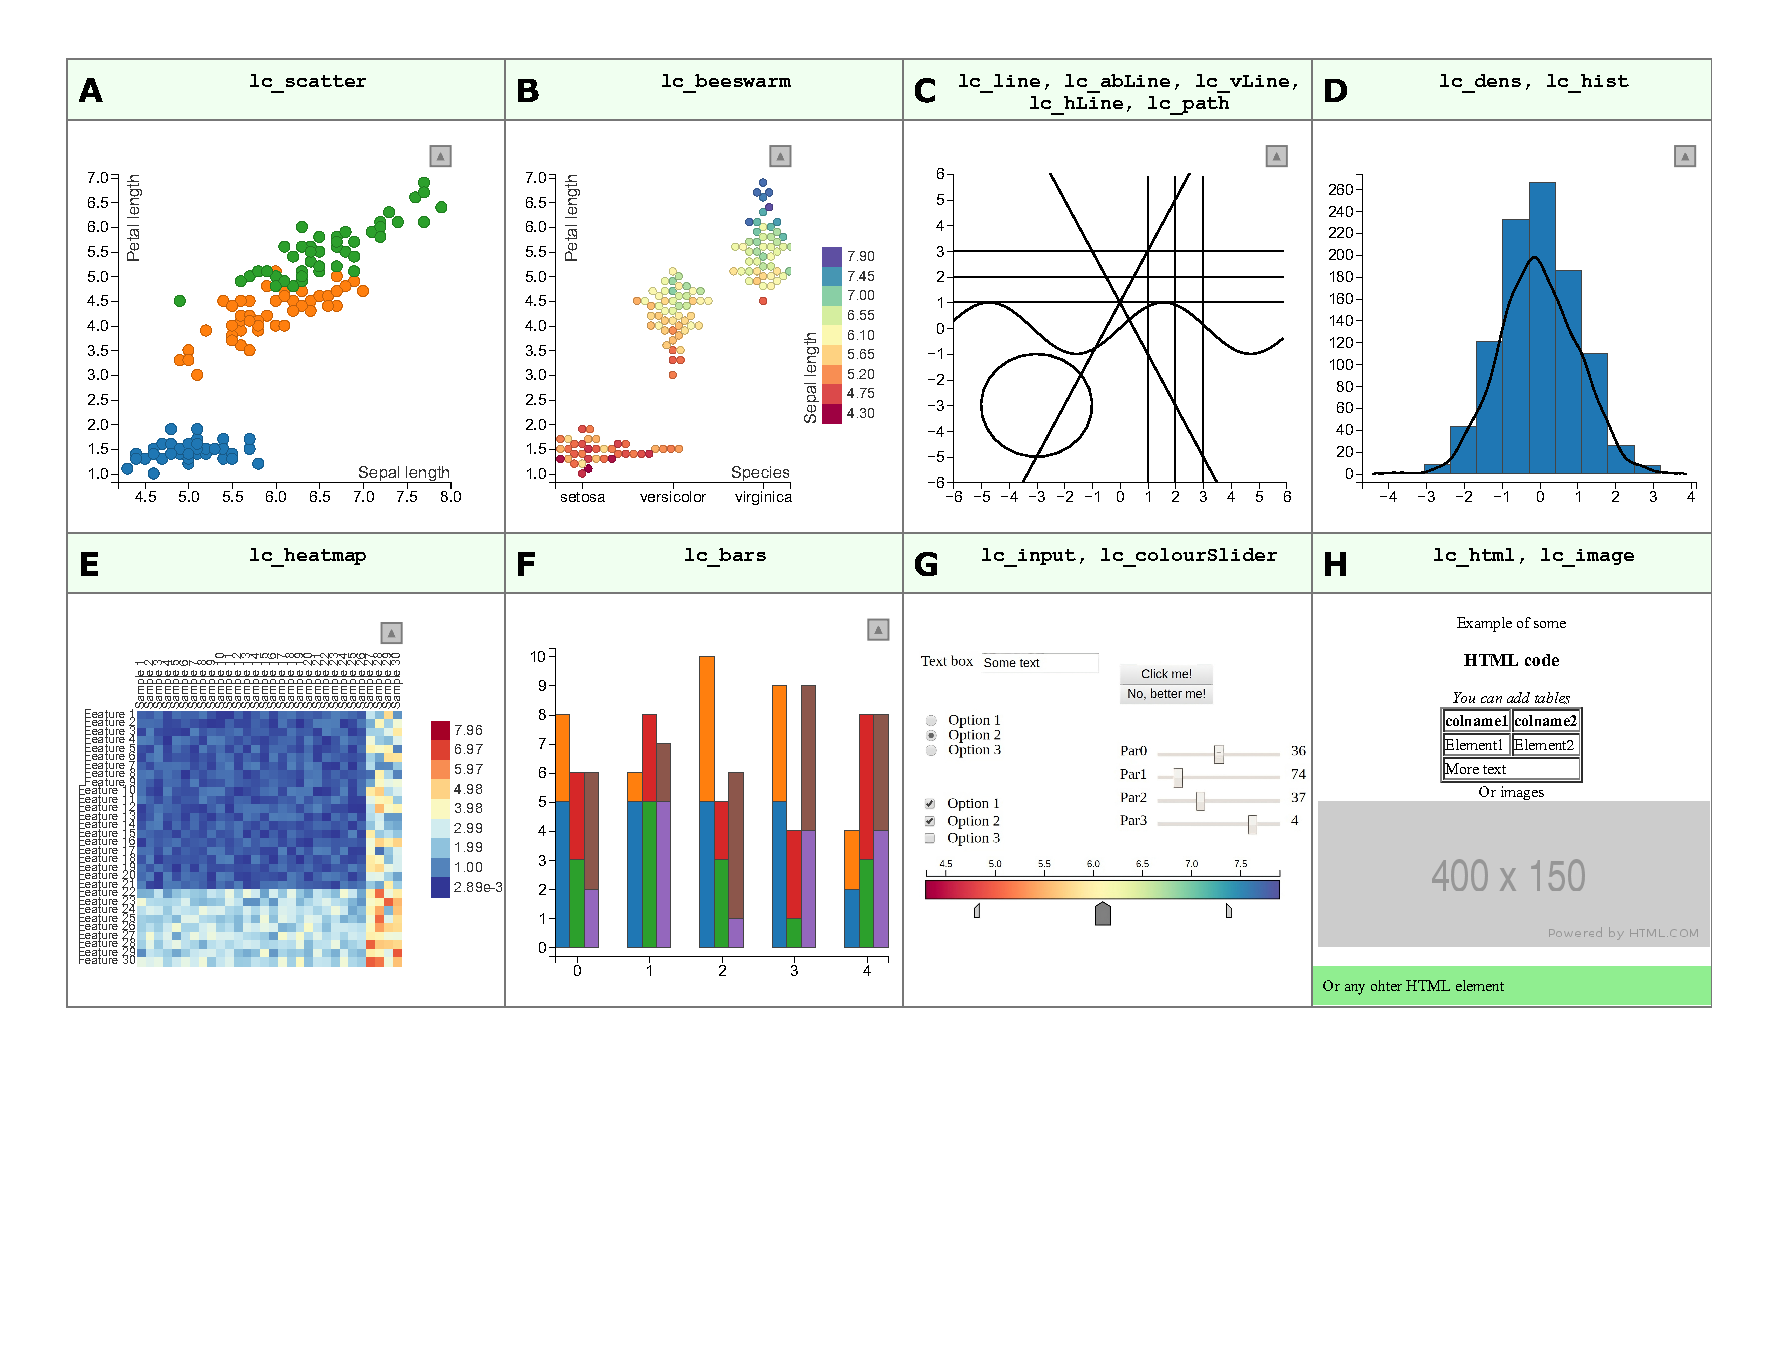
\includegraphics[width=\textwidth]{FigA/figA.png}
	\caption{Gallery of all available plotting functions the in \mintinline{R}{rlc} package. A scatter plot (a); a bee swarm plot (based on d3-beeswarm plugin [reference]) (b); a collection of various line plotting functions (c); a histogram and a density plot (density was multiplied by a factor of 500 to be visible on the same plot as the histogram) (d); a heatmap (e); a bar chart (f); a collection of elements to gather input from user (g); a function to add custom HTML code to the page (h). All this examples with code to create them can be found in the supplement.}
	\label{FigA}
\end{figure*}

R/LinkedCharts syntax is very similar to most commonly used plotting libraries. There is a set of 14 main functions - each responsible for a specific type of chart (such as scatter plot, heatmap, bar plot, etc.) or a navigation element (such as sliders or text fields). Figure \ref{FigA} shows them all together with some basic examples. Each plot is defined by its properties: some of them are required (such as \mintinline{R}{x} and \mintinline{R}{y} for a scatter plot or \mintinline{R}{value} for a heatmap) many others are optional (\mintinline{R}{palette}, \mintinline{R}{title}, \mintinline{R}{ticks} etc.). A full list of all the properties with live examples is available at \url{https://anders-biostat.github.io/linked-charts/rlc/tutorials/props.html} and also on the R man page for each plotting function. Many of the properties accept minor variations in spelling (\mintinline{R}{colour/color} or \mintinline{R}{labels/label}).

\begin{figure*}
	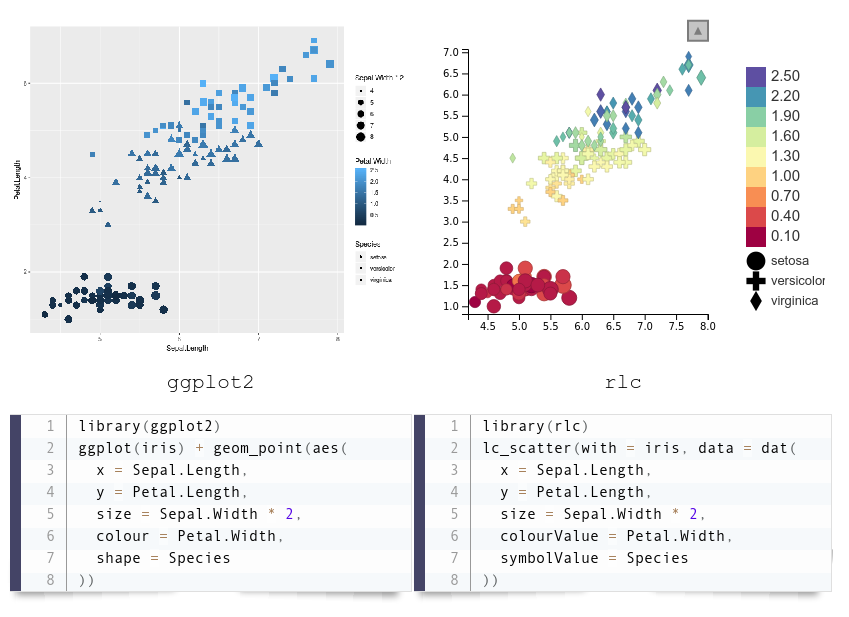
\includegraphics[width=\textwidth]{FigB/figB.png}
	\caption{Typical syntax of a R/LinkedCahrts plot and its comparison with ggplot2 [ref] library as an example of one of the most commonly used plotting libraries. Lines of code are arranged so that same aspects of the charts are set next to each other. ``iris'' dataset, which is one the R built-in datasets, was used for this example. Both pieces of code are fully functional and their output is shown above the code.}
	\label{FigB}
\end{figure*}

The same structure with some minor differences in syntax is used in many generally used plotting libraries. For instance, in Figure \ref{FigB} a comparison between \mintinline{R}{ggplot2} and \mintinline{R}{rlc} syntax is shown for making a simple scatter plot. As one can see, there is hardly any differences there. An important thing to notice here is the \mintinline{R}{dat} function, which plays the key role in R/LinkedCharts. Any property, defined inside this function, can be reevaluated at any moment simply by calling the \mintinline{R}{updateCharts} function. The corresponding plot will be then redrawn accordingly to the current state of the environment.

To make it more clear, let us imagine that we have a matrix \mintinline{R}{countMatrix} with some single-cell RNA-seq experiment results. Each row of the matrix is a gene, each column is a cell and values are numbers of reads from given gene detected in a given cell. Now we want to plot gene expression in two cells against each other and we have index of one of them stored in a variable named \mintinline{R}{cell1} and of the second one in \mintinline{R}{cell2}. To do this in R/LinkedCharts one should write the following code:

\begin{minted}{R}
lc_scatter(dat(x = countMatrix[, cell1], 
   y = countMatrix[, cell2]))
\end{minted}

If now values of \mintinline{R}{cell1} and \mintinline{R}{cell2} are changed, calling the \mintinline{R}{updateCharts} function will change the scatter plot to show gene expression in these new cells. The only thing that is missing now to make an interactive app is a reaction to mouse events on the web page. To this end, R/LinkedCharts provides a set of callback functions for the most common mouse events. They are all arguments with names spelled as \mintinline{R}{on_`eventName`} and a list of available listeners can differ between different chart types. A full list can be found on R man pages for each plotting function.

The most often used callback function is \mintinline{R}{on_click}. It is called every time an element of a chart (point, line, bar, cell) is clicked. A an argument this function gets index of the clicked element or two indices - for a row and a column in case of a heatmap. Let's extend our example to demonstrate the use of the \mintinline{R}{on_click} callback. Based on the above mentioned \mintinline{R}{countMatrix}, we can calculate some distance or correlation matrix to explore cell-to-cell similarities. For demonstration purposes, distances can be obtained in a very straightforward manner.

\begin{minted}{R}
distMatrix = as.matrix(dist(countMatrix))
\end{minted}

Now, next to the scatter plot of gene expressions in the two selected cells, we can have a heatmap of distances which is also used for navigation through all the pairs of cells. 

Code for such a minimalistic, but already fully functional interactive app is presented below:

\begin{minted}{R}
lc_heatmap(value = distMatrix, 
   on_click = function(d) {
      cell1 <<- d[1]
      cell2 <<- d[2]
      updateCharts()
})
lc_scatter(dat(x = countMatrix[, cell1],
	y = countMatrix[, cell2]))
\end{minted}

You can find the app produced by this code in the supplement alongside with a more nicely looking version.

In this example we use the \mintinline{R}{on_click} callback function to change the state variables \mintinline{R}{cell1} and \mintinline{R}{cell2} and to redraw the scatter plot. As it was previously mentioned, properties \mintinline{R}{x} and \mintinline{R}{y} will be reevaluated using the current values of the state variables, thus making it easy to keep charts up-to-date and ensure interactive behaviour.

This basic example illustrates the main idea behind the LinkedCharts library. We define a set of charts employing a collection of variables to specify current state of the chart, i.e. selected cells, genes, samples, color labels, etc. With the help of the mouse event callback functions we change the state variables and call the \mintinline{R}{updateCharts} function to put the charts in accordance with their new values. This process is what "linked" in "LinkedCharts" stands for. We link several charts together by the means of \mintinline{R}{on_click} and other callback functions and updating charts. Though quite simple, this structure can produce powerful interactive apps for various research purposes.

The app from the example can be further customized by changing colours, shapes and sizes or adding meaningful labels and titles. Some technical aspects can be changed as well for better performance. For instance, we can specify what exactly should be redrawn on each \mintinline{R}{updateCharts} call and prevent meaningless updates of the heatmap. Please, check the supplement for a prettified version of the app with all necessary explanations.

\subsection{Use Cases}
\subsubsection{Quality check}

It is common that on the way from obtaining raw data towards meaningful conclusions one undertakes a number of steps each involving some data condensing and inevitable information loss. For example, raw reads in RNA-seq are aligned and counted to produce a gene expression levels for each sample. However, quality of reads and confidence of alignment is no longer included in the data. If now researcher is interested in clusters of samples and other patterns such as trajectories, the next step may be to calculate a distance matrix. This will make data even more interprateable, but now we loose gene expression values. Of cource, various steps are performed on each step. Low-quality reads are usually removed from the study as well as samples that show weird expression patterns. We tend to beleive that we now longer care about those pieces of data that are left behind in the research flow, since we've already taken everything we need from them.

\begin{figure*}
	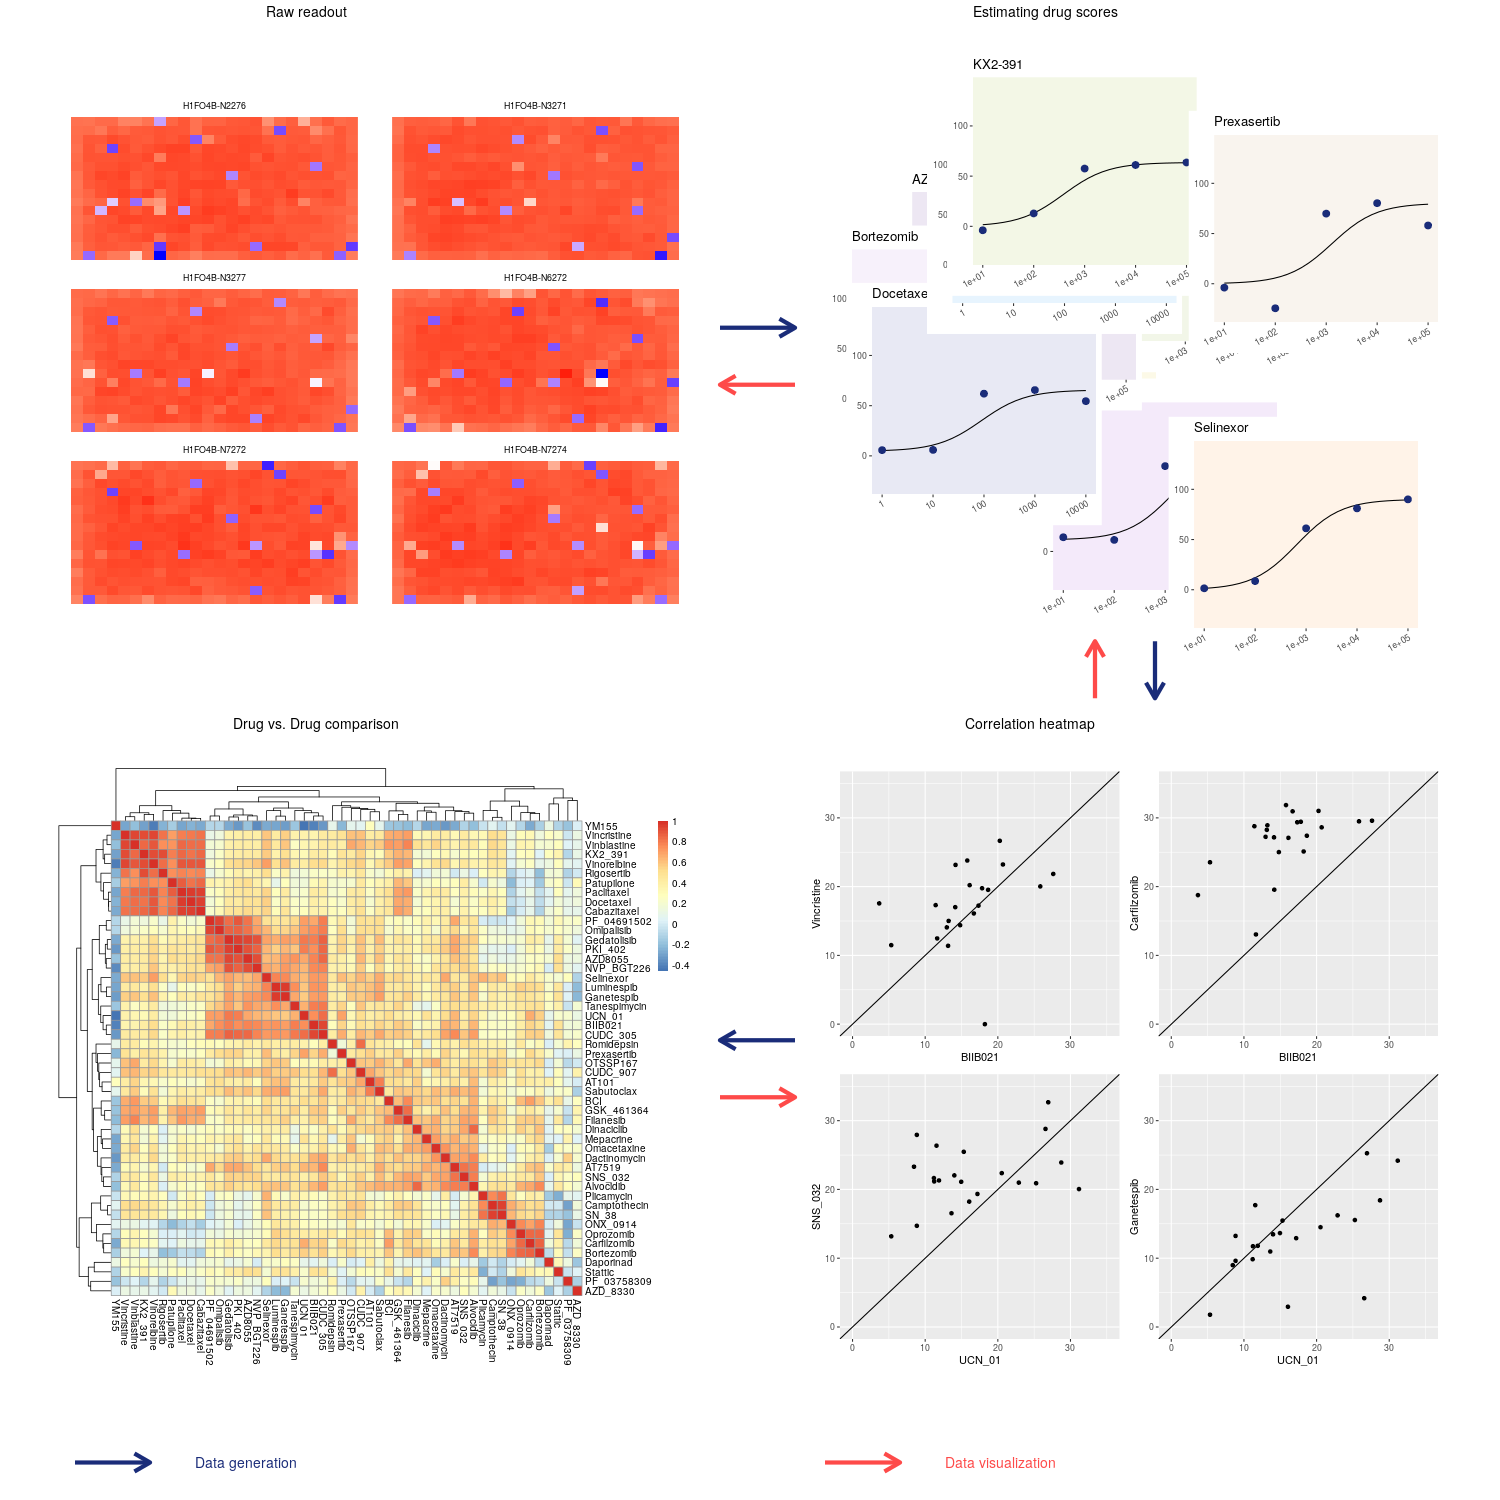
\includegraphics[width=\textwidth]{FigC/figC.png}
	\caption{}
	\label{FigC}
\end{figure*}

However, it is always good to check whether an intresting pattern that one observes in a 2D embedding is a real finding or a technical artifact of some sort. Generally, it requieres taking one or several steps back, retrieving only the data that is related to samples in question, making some new plots. All this can be easily done with a Linked-Charts app.

The idea is to make a chain of charts, where each new one explains each element of the previous one. For example, in the app from the previous section, scatter plot explains each cell of the heatmap. When a cell is clicked, we can see all the expression values for the two selected samples and thus it "explains" the obtained distance value. We can continue the chain of charts and, for instance, add a chart that for a selected gene will show quality of reads all the reads for the two selected samples.

Such an app would allow a quick and easy spot check of uncovered data patterns and can give researcher a better way to understand inner connections between the data. Such as to what extent noise cab influence the signal or what scale of changes in the value of interest is typical to the data.

Another example is given in the supplement. It is based on the data from a drug-screening experiment where a panel of (??) drugs was tested against pancreatic cancer cell lines (??). The main heatmap shows drug-drug correlation. By clicking on a cell of the heatmap user selects to drugs and can check individual inhibition levels of each of them against all the tested cell lines. The inhibition values were calculated based on drug activity in five tested concentrations and on the third plot one can check all those activity levels for each conentration. More details as well as code and links to download the data one can find in the supplement.

\subsubsection{Exploratory analysis}
To emphasize the simplicity of the Linked-Charts library, for every example in supplement we provide two versions. One contains bare minimum of code to produce working and useful app. This kind of apps can be easily written on-the-fly to facilitate current research steps. The other shows how to make those work-in-progress-apps more presentable. This, usually, takes more effort, but not much more than to prepare a usual static plot for a paper of a presentation.

Syntax of Linked-Charts is made as simple and as similar to syntax of commonly used plotting libraries to urge researchers to employ interactivity for every-day exploration analysis. We beleive that one doesn't need to wait for special occasion or some final results to start playing with interactivity. Instead, interactive apps can be made as often and easily as static plots. For example, if you are performing some differential expression analysis and want to make an MA-plot, it may be reasonable to always have a plot showing individual expression levels next to it. It takes just a few extra lines of code, yet provides a whole layer of useful information.

Here, how one can make these two linked plots using the Linked-Charts library (more details and used data can be found in supplement).

\begin{verbatim}
openPage(layout = "table1x2")

gene <- 1

lc_scatter(dat(
x = voomResult\$AveExpr,
y = voomResult\$tissuetumour,
on_click = function(k) { gene <<- k; updateCharts("A2") }),
"A1")

countsums <- colSums(countMatrix)

lc_scatter(dat(
x = sampleTable\$patient,
y = countMatrix[gene,] / countsums * 1e6 + .1,
logScaleY = 10),
"A2")
\end{verbatim}

This example is very similar to the one from the previous section, but we've added the `openPage` function to set a table layout to the web page. This step is optional and allows us to put the two charts next to each other.

\subsubsection{Server apps}
Linked-Charts apps can be used locally by the researcher and can also be shared as sever apps. And there is only one additional thing that is required to turn local app into a server app: One needs to specify a list of local variables and their default values. Local variables are ones that can be rewritten by several users independently. In most cases they are also state variables: i.e. variables that store current state of an app (selected genes, samples, etc.). Thus, to run the app from the previous section, one would need just to replace the first two lines with
\begin{verbatim}
openPage(layout = "table1x2", sessionVars = list(gene = 1))
\end{verbatim}

Now the app can be accessed by multiple users simultaneously.

Of course, there are other things that can make a server app more customized. One can add some default content to each opened page, control each client session (and, for example, close those, that don't show any activity for considerable amount of time), limit memory usage or number of active connections simultaneously. Yet, all these parameters are optional.

\subsubsection{Stand alone apps}
Linked-Charts can also be used to create stand-alone apps. For this kind of apps you don't need a server, but can directly send them to a collaborator as an HTML file that can be opened in any browser. The page will already contain all the data and interactive functionality. Yet to make such an app one should use a JavaScript version of the Linked-Charts library. We tried to make required level of experience with JavaScript to minimum and make necessary code understandable. For each example in the supplement we also provide the JavaScript code necessary to create the same app without running R session. More documentation on linked-charts.js as well as various tutorials are available at...

\subsection{Further customization}



\end{document}


